\chapter{Design}
\label{chapter:design}

\section{Software Architechture}
\label{sec:software-architechture}

In this section we will discuss the software architecture of the system. We will present the MVC architecture that will be used for the system. The interaction between the components will be discussed in detail. Figure \ref{fig:architechture} shows an overview of the software architecture of the system.

\begin{figure}[!ht]
    \centering
    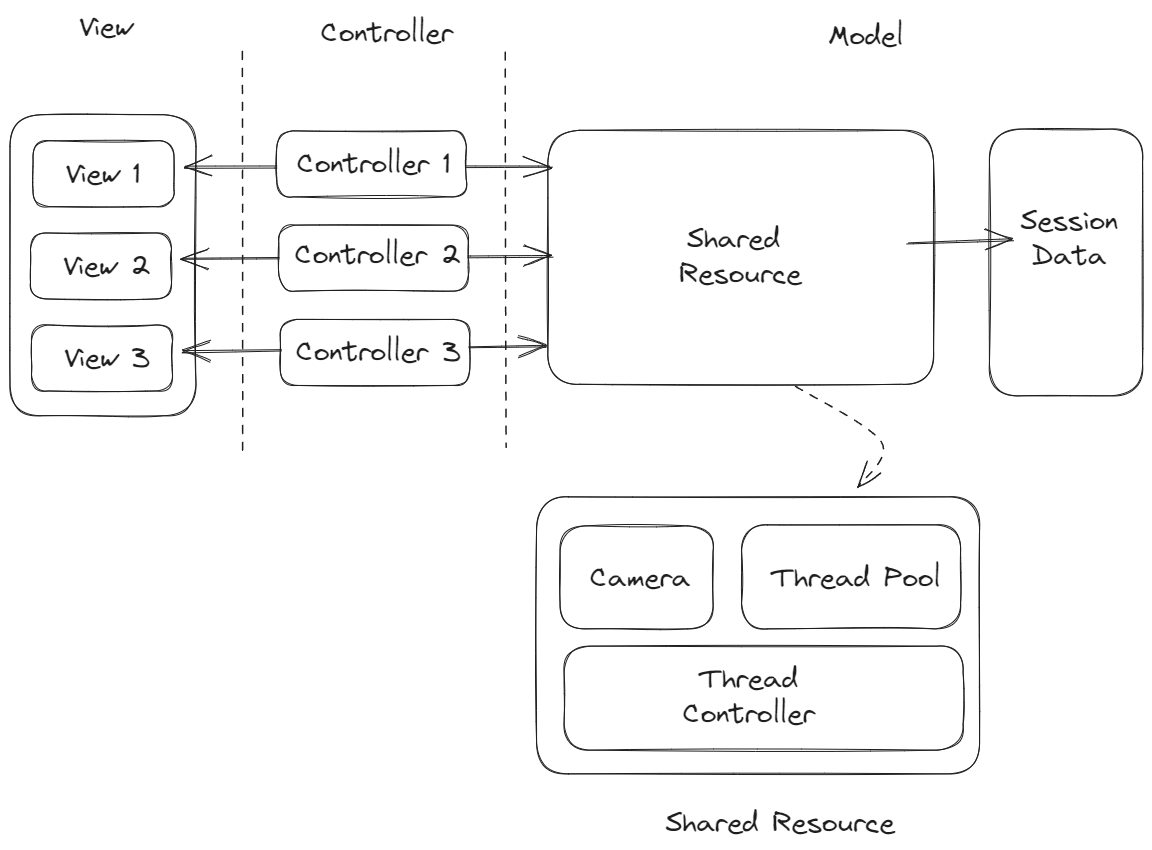
\includegraphics[width=0.8\textwidth]{texs/Part2/chapter3/image/architecture.png}
    \caption{Software Architecture}
    \label{fig:architechture}
\end{figure}

\subsection{Model-View-Controller}
\label{subsec:model-view-controller}

The implementation of the Model-View-Controller (MVC) architecture in this system is depicted in the accompanying figure. One key aspect to highlight is the complete decoupling of the model and view, both of which are under the strict control of the controller. When an input is provided to View 1, Controller 1 takes charge, handling the request and orchestrating interactions with the model. The resulting response is then seamlessly relayed back to the view, conveying the status of the request, be it success, failure, or otherwise.

Notably, the view components are meticulously separated from one another. This deliberate segregation prevents any unintended mixing of view elements. For instance, View 1 might necessitate specific UI components, while View 2 might require an entirely different set. This simplifies the implementation process and renders it more comprehensible.

Furthermore, the controller components are also discretely compartmentalized. As illustrated, Controller 1 and Controller 2 are each affixed to their respective views. Additionally, there exists a shared resource component that interfaces with the controllers. This design strategy aims to circumvent the predicament of a "Giant Controller" problem, as discussed earlier. Consequently, developers can more readily discern the controller's core responsibility, which is to mediate the flow of requests and responses between the model and view. Any other pertinent business logic is appropriately handled within the shared resource area, as expounded upon in the subsequent section.

For this system, a conscious decision was made to adopt a shared model approach, in contrast to isolating controllers or views as distinct entities. This shared model approach facilitates the seamless exchange of data among various components. By doing so, it is anticipated that data management will be more straightforward and cohesive. The paramount consideration is ensuring that robust data handling procedures are in place, guaranteeing that the data remains consistently updated.

This design philosophy is underpinned by a commitment to scalability. By vertically stacking views and controllers, the addition of new views becomes a streamlined process. To accommodate a new view, a corresponding controller is introduced and connected to the model, thus fortifying the system's scalability and adaptability.

\subsection{Thread Pool}
\label{subsec:thread-pool}

For this project, the thread pool object will play a pivotal role in improving the efficiency of the system. The thread pool object will be responsible for managing the threads that are used to execute the tasks, as discussed previously in Chapter \ref{sec:thread-pool}. It solve one of the problem mentioned in \cite{Sabtu_2023}, where some computer vision algorithms are computationally expensive and can take a long time to execute.

If these tasks are to be run in single threaded execution, the user will have to wait for a long period of time before the task is completed. This is not ideal for a user interface application, as it will cause the application to be unresponsive. However, if multiple of this instances are to be run in parallel, it will cause the system to be overloaded and can cause the system to crash.

This is where the thread pool comes in to solve this problem. It will create a fixed number of available threads, which allows for parallelism but also prevents the system from being overloaded. The thread pool will also manage the threads, which means that the user does not have to worry about creating and managing the threads. The user only needs to create the task and submit it to the thread pool, which will then assign the task to an available thread.

\subsection{Thread Controller}
\label{subsec:thread-controller}

The Thread Controller is a critical component introduced to alleviate the responsibilities of the main controller in a system. By incorporating a Thread Controller, the main controller can focus on efficiently handling requests between the view and the model, without becoming bogged down with intricate threading operations.

Within the Thread Controller, there exists multiple sets of threads. It's important to note that these threads are distinct from those defined within a thread pool. In this context, the threads within the Thread Controller are specialized units responsible for executing specific business logic. Each thread operates in parallel, enabling the system to handle multiple tasks simultaneously.

Moreover, the Thread Controller is designed with access to a Thread Pool. This integration empowers the system to execute tasks that necessitate parallel processing in an organized manner. Tasks can be placed in a queue within the Thread Pool, ensuring they are executed efficiently and without resource conflicts.

This implementation stands as a powerful facilitator of scalability. Developers have the flexibility to define their own sets of threads, tailoring the system to meet specific performance requirements. Additionally, Developers gain the ability to exercise fine-grained control over thread execution directly from the controller, promoting a high degree of customization and adaptability to varying workloads. This dynamic combination of a Thread Controller and Thread Pool lays a robust foundation for responsive, efficient, and scalable applications.


\section{User Interface Design}
User Interface (UI) design is a crucial aspect of product development that focuses on the look, style, and interactivity of a product \cite{Coursera_2023}. It is the first thing users encounter when they use an application or visit a website \cite{Coursera_2023}.
A user-friendly UI design holds a pivotal role in enriching the user experience, boosting user engagement, and ultimately shaping the success of an application \cite{AlgoRepublic_2023}.

There are various design guideline that can be utilized in order to create a user-friendly UI design. Paun \cite{Paun_2020} stated that, familiarity in UI design benefits both users and designers. It streamlines workflows, ensures a seamless experience, and allows for efficient use of established conventions. Adhering to standards and maintaining consistency are key for a unified and positive user experience.

Fleck \cite{Fleck_2021} argues that, simplicity in design plays a crucial role in UI design.  A simple design minimizes cognitive load and allows users to accomplish tasks efficiently. The author also emphasize that it is important to remember that simplicity does not mean sacrificing functionality; rather, it means prioritizing essential elements and removing any extraneous details that may cause confusion or overwhelm the user.

In GUI design, feedback is as important as consistency and simplicity. It comes in forms like visual cues and error messages, helping users understand the product's state and how to interact with it. This feedback lessens confusion, builds trust, and aids in learning how to use the product, even when errors occur. \cite{Florido_2022}

\subsection{Wireframe}
\label{subsec:wireframe}

Wireframing is the first step in UI design \cite{Gupta_2023} \cite{Chen2020} \cite{Rahmadi2020}. A wireframe is a basic, simplified layout of a digital interface that outlines content placement and page components \cite{White_2023}. It serves as a quick way to present a concept or idea without extensive time or resources \cite{White_2023}.

Gupta \cite{Gupta_2023} stated that, a good wireframe abstains from including elements that could divert attention from decisions pertaining to the site's structure, but it instead prioritizes the functional purpose over visual aesthetics, presenting a straightforward, unadorned portrayal of the website's features in monochrome. The  author also stated that, designers should provide annotations to explain and elaborate on specific features, providing clarity and context.

Figure \ref{fig:wireframe} shows the rough sketch of the user interface that will be used for this project. The user interface will be divided into 4 main sections: the title panel, image panel, status panel, and button panel.

\begin{figure}[!ht]
    \centering
    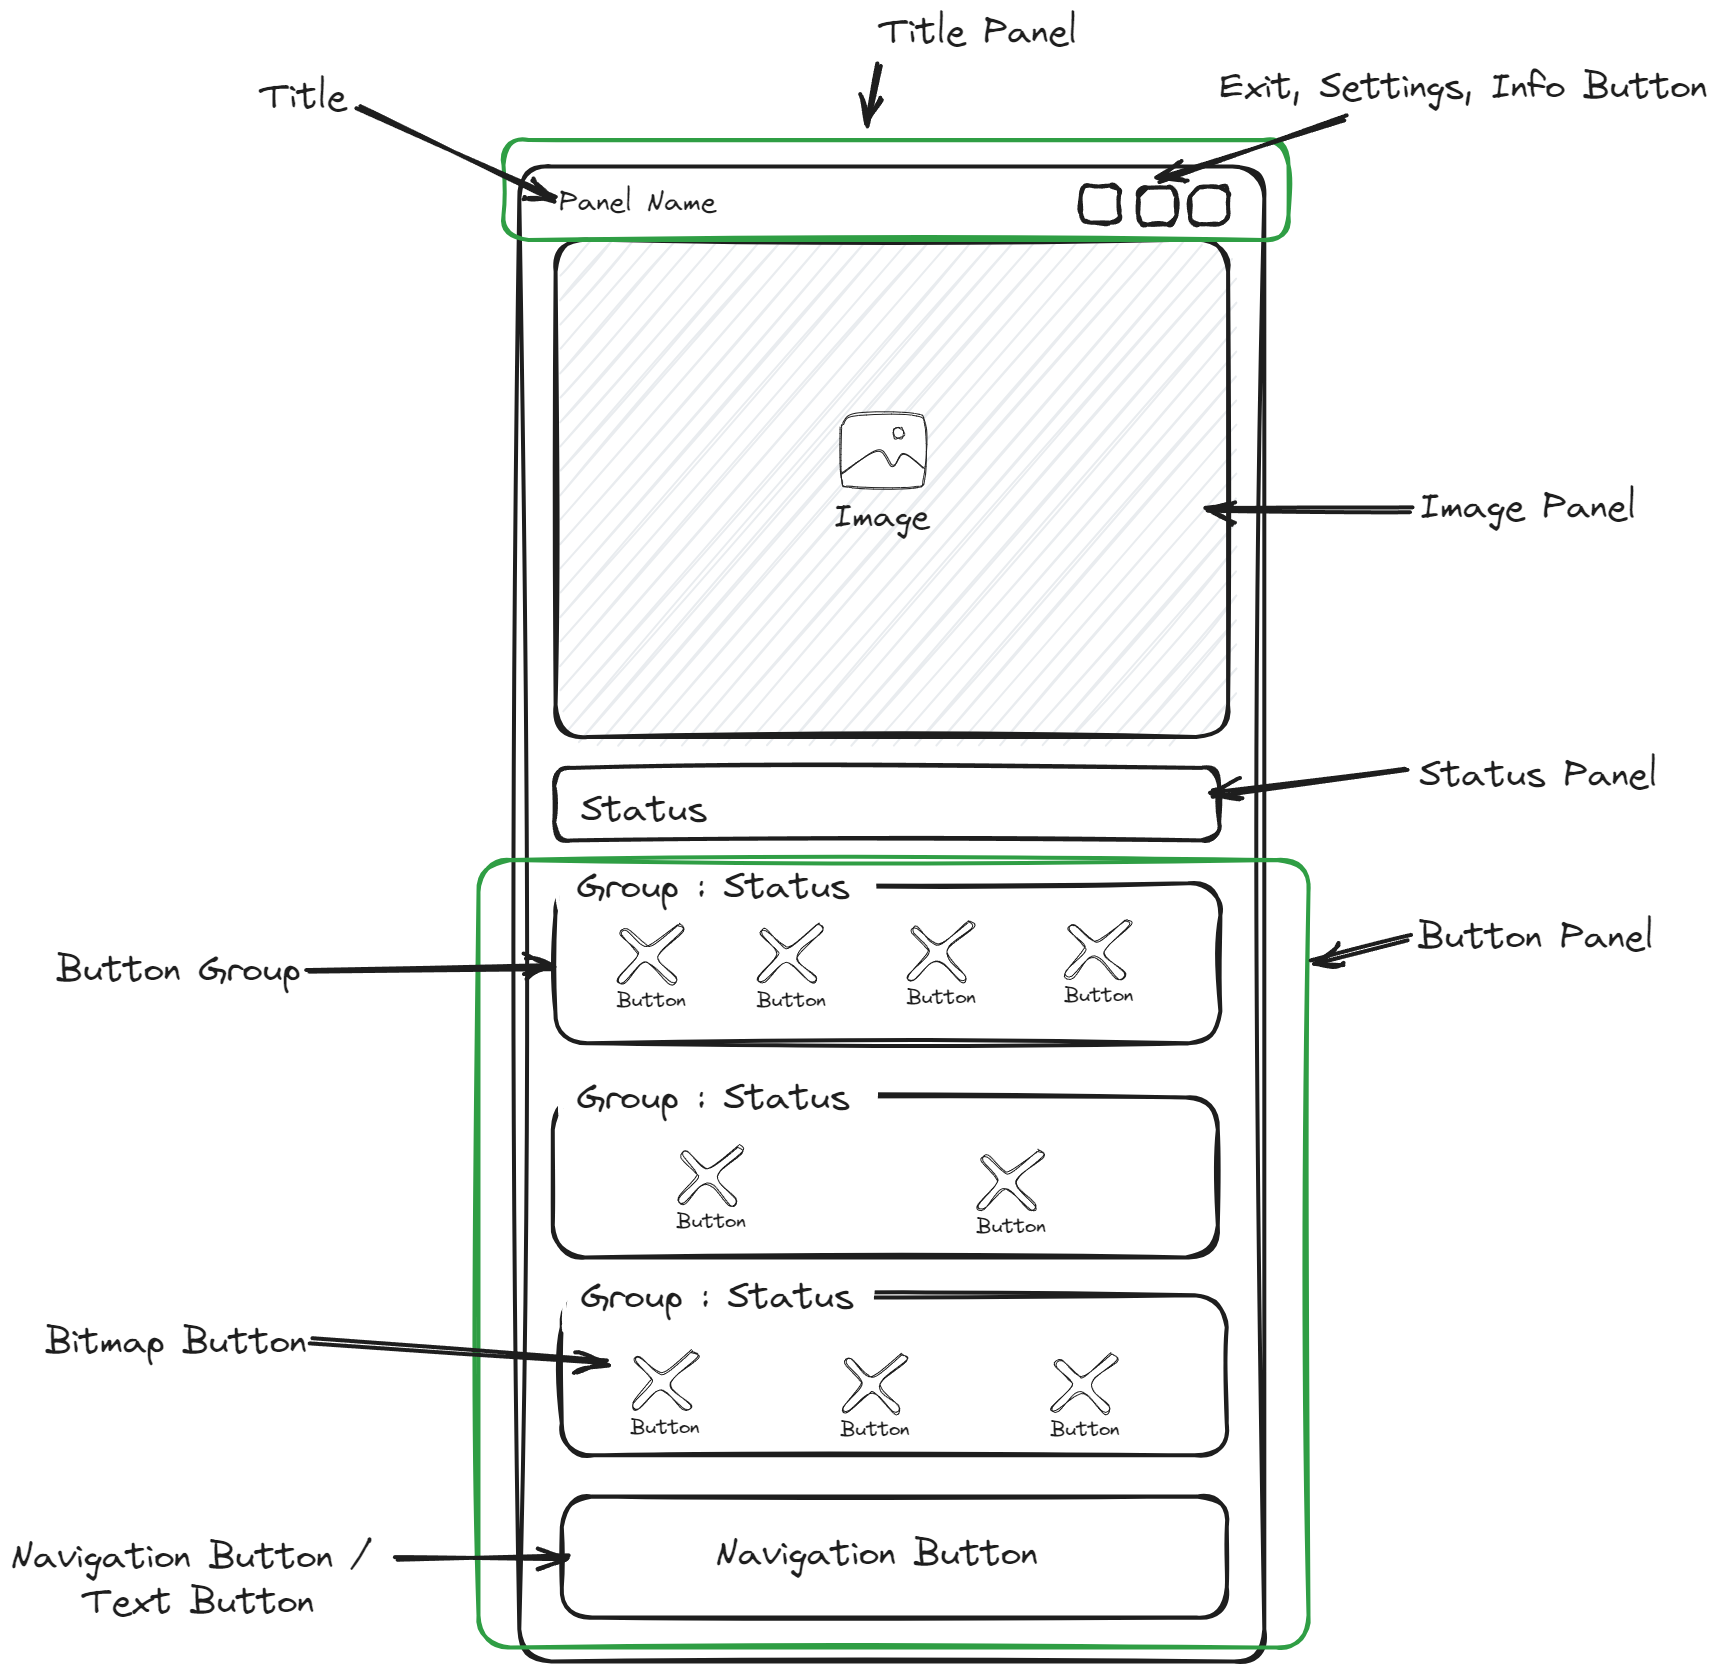
\includegraphics[width=0.65\textwidth]{texs/Part2/chapter3/image/wireframe.png}
    \caption{Wireframe}
    \label{fig:wireframe}
\end{figure}

The title panel will be used to display the title of the application. It provide information to the user on which panel they are currently in. Additionally this component also provide other functionality for user such as closing the application, accessing the setting, and provide some basic information on the application.

The image panel is purposed to display images to user. It will be used to display the image that is captured by the camera, and also the image that is being processed. The status panel will be used to display the status of the application to the user. It is important to provide feedback to the user on the status of the application, so that the user will know what is happening in the application.

The button panel will be used to display the buttons that the user can interact with. In this panel, buttons will be grouped into its own categories, depending on its functionality. There will be two types of buttons in this panel, which are the bitmap button and the text button.

\subsection{Mockup}

something something

\subsubsection{Color Scheme}

Color is a pivotal element in UI design, playing a vital role in evoking emotions, establishing hierarchy, and distinguishing design components \cite{M._2023}. When employed adeptly, color can greatly improve the usability and overall user experience of your website or mobile application \cite{M._2023}.

Ou et al. \cite{Ou04} emphasized the strong correlation between color and emotion, highlighting how different colors evoke specific emotional responses. Their research underscores the significant impact that color choices can have on the emotional experience of users.

Lewandowska and Olejnik-Krugly \cite{Lewandowska2021} emphasized that color is a significant aspect of visual communication, playing a vital role in conveying information. It is integral in identifying products, indicating quality, and influencing user interfaces.

They also stated that, colors can evoke diverse visual sensations, and their impact is often experienced in combination rather than in isolation, at which it underscores the intricate role of color in human perception and communication.

Zhang and Ferris \cite{Zhang16} discusses factors for choosing colors in design: number of colors, color harmony, and text overlay. For the number of colors, options range from a single color with various shades to a 60-30-10 rule for triadic schemes, emphasizing primary, secondary, and accent colors. Figure \ref{fig:color-scheme} shows a few examples of color combination with 60-30-10 rule.

\begin{figure}[!ht]
    \centering
    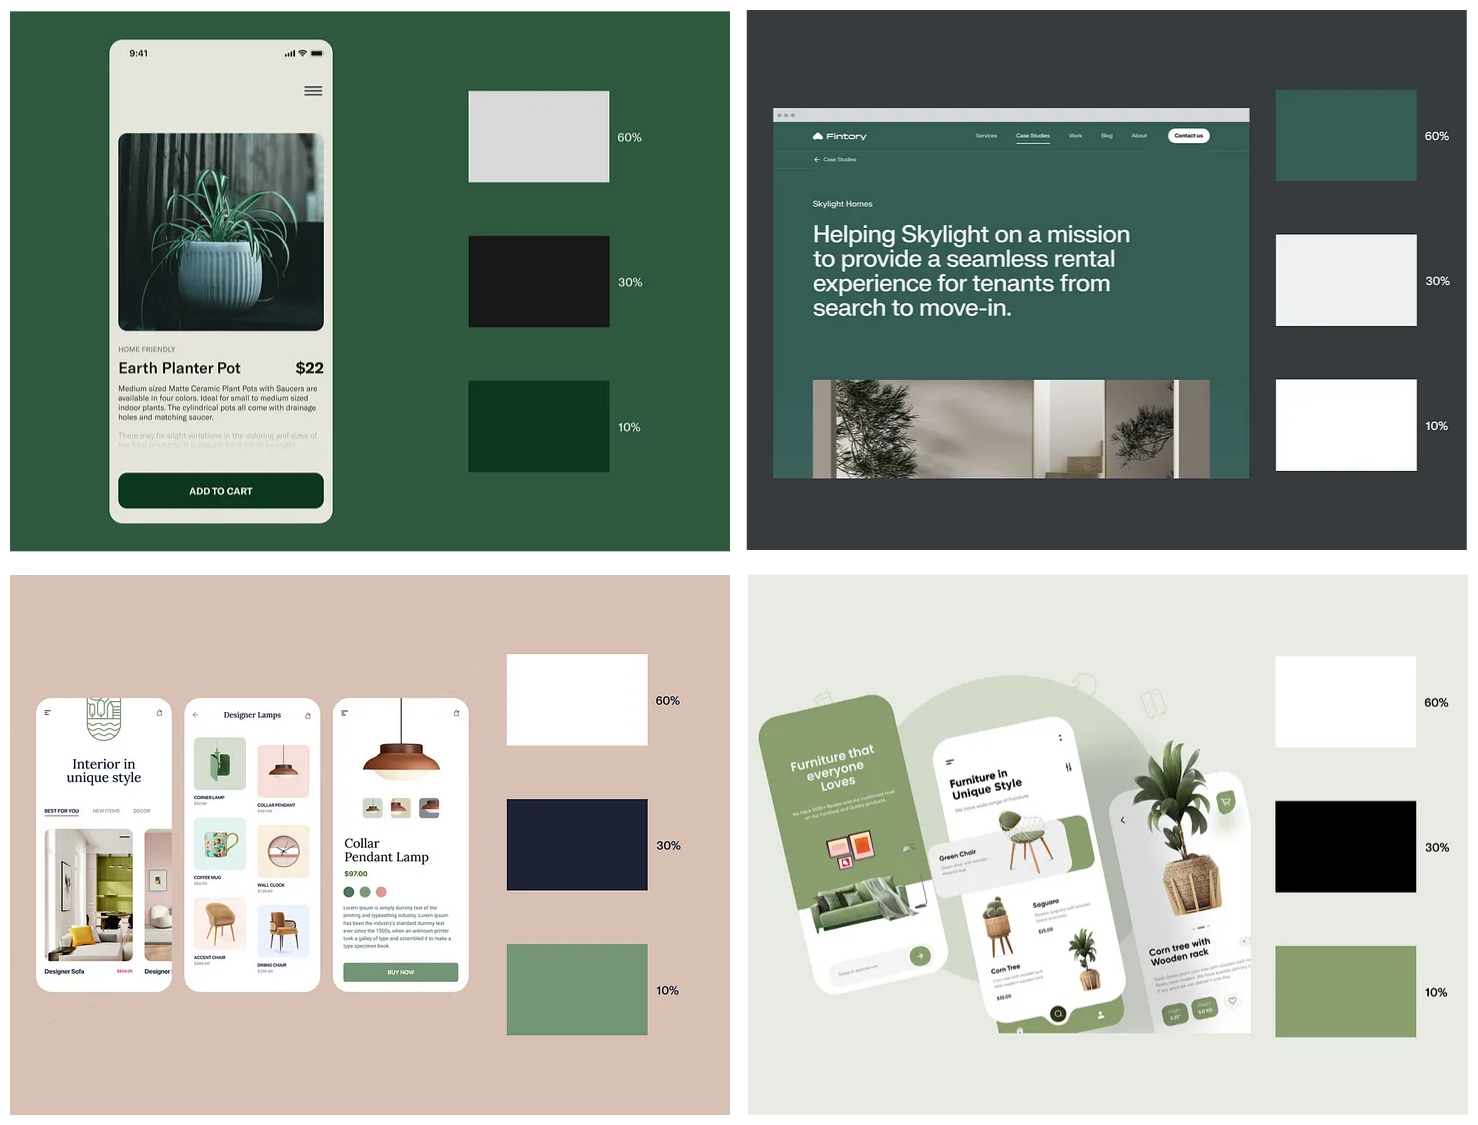
\includegraphics[width=0.8\textwidth]{texs/Part2/chapter3/image/colorexample.png}
    \caption{Example of Color Combination with 60-30-10 Rule \cite{M._2023}}
    \label{fig:color-scheme}
\end{figure}

In choosing the primary color, it is important to consider the brand's message and the emotions that the brand wants to evoke \cite{M._2023}. The secondary color should complement the primary color and provide contrast to support the dominant color, while the accent color is used in features like buttons and pop-ups  \cite{M._2023}.

Figure \ref{fig:color-combination} shows the color combination that will be used for this project. A simple white and black color combination is used for the primary and secondary color respectively. Since the target user will be the policemen, the blue shade is used for the accent color to represent the police force.

\begin{figure}[!ht]
    \centering
    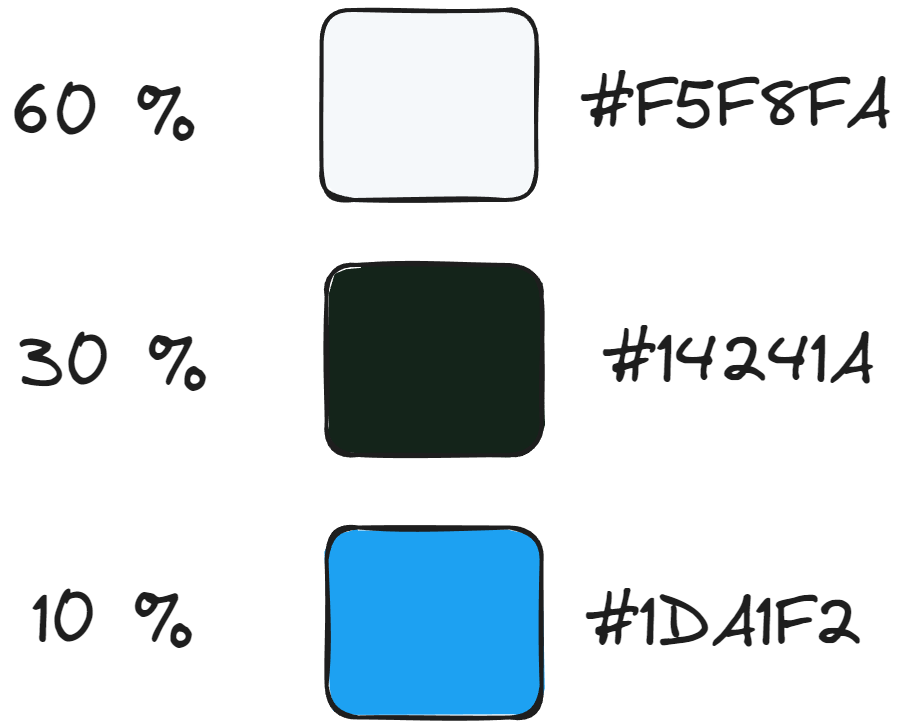
\includegraphics[width=0.45\textwidth]{texs/Part2/chapter3/image/colorcombination.png}
    \caption{Color Combination}
    \label{fig:color-combination}
\end{figure}

\subsubsection{Typography}
Typography is a critical element in UX design, as over 90\% of online information is presented in text form \cite{Fitz-Patrick_2022}. It involves more than just selecting attractive fonts and other factors such as typeface, font, character, baseline, and height are important \cite{Fitz-Patrick_2022}.

Sawyer \cite{Sawyer2020} stated that, picking the right font is really important. It affects how things look and how easy they are to read. This is especially true for quick glances on screens. Recent studies found that different fonts can make a big difference in how easy things are to read in real-life situations.

For this project, the font that will be used is Roboto. Roboto is a sans-serif typeface family developed by Google as the system font for its mobile operating system Android \cite{Mott_2022}. According to Google, this font is optimized to provide optimal reading experience across various devices \cite{Mott_2022}. Figure \ref{fig:roboto} shows the Roboto font that will be used for this project.

\begin{figure}[!ht]
    \centering
    
\includegraphics[width=0.4\textwidth]{texs/Part2/chapter3/image/roboto.png}
    \caption{Roboto Font}
    \label{fig:roboto}
\end{figure}










